\section{System Layer and Interactive Access}
\label{sec:system-layer}

An embedding survey is substantially more useful when readers can move from the paper to a runnable interface. For that reason, this repository includes a lightweight Leaflet-based prototype that consumes the structured dossier and presents four elements in a single view: a model selector, a pilot region of interest, runtime metadata, and task-oriented interpretation notes.

The intended system architecture has three layers. The first layer stores model metadata, processed paper notes, and benchmark outputs. The second layer exposes embedding extraction, product sampling, and export services behind a uniform API. The third layer provides the browser interface for region selection, model comparison, and rapid task setup. This structure mirrors the logic of the review itself: concepts and model metadata first, benchmarking second, and access tooling third.

\begin{figure}[t]
  \centering
  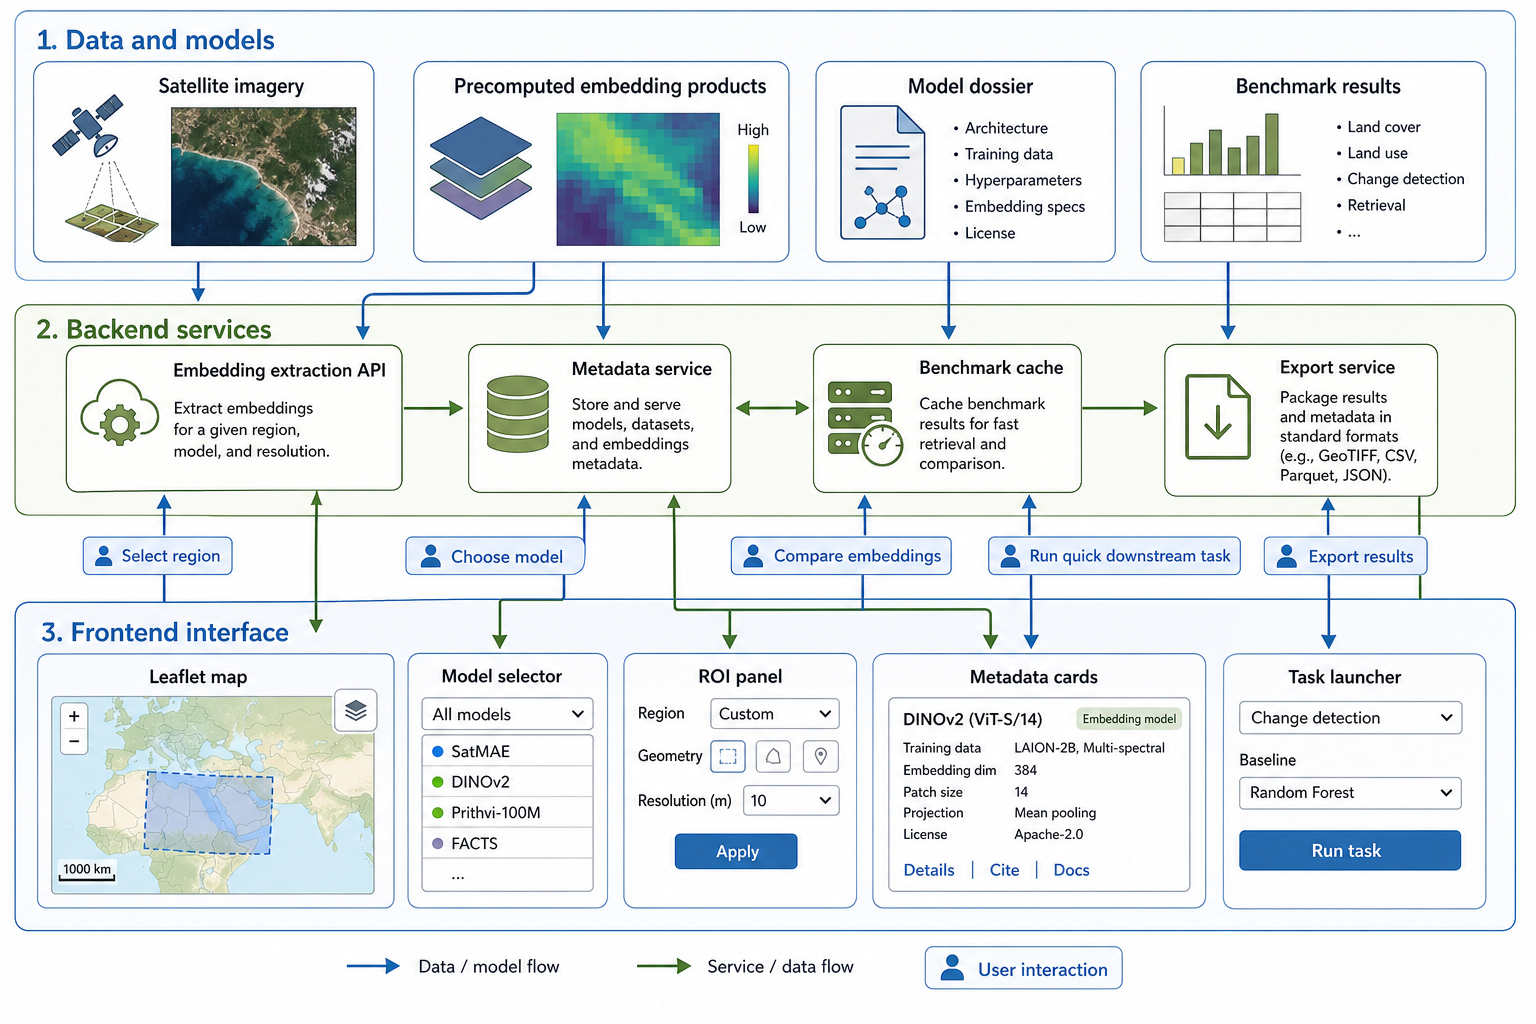
\includegraphics[width=\textwidth]{fig03_system_overview_gptimage2_20260502.png}
  \caption{System layer for the proposed Satellite Embedding Explorer. The same structured assets used by the review can also drive metadata browsing, ROI selection, model comparison, and later benchmark services.}
  \label{fig:system-overview}
\end{figure}

Even the current static prototype is useful because it forces the review assets into machine-readable form. The same \texttt{model\_dossier.json} file can drive paper tables, browser filters, and later benchmarking scripts. This reduces duplication and makes it easier to keep the literature summary synchronized with the software layer.
